\chapter{Исследовательская часть}

В данном разделе будут приведены примеры работы программ, постановка эксперимента и сравнительный анализ алгоритмов на основе полученных данных.

\section{Технические характеристики}

Технические характеристики устройства, на котором выполнялось исследование.

\begin{enumerate}
	\item Операционная система: Windows 10 Корпоративная, Версия	21H1, Сборка ОС 19043.2006.
	\item Память: 8 ГБ.
	\item Процессор: AMD Ryzen 5 4600H с видеокартой Radeon Graphics \\3.00 ГГц \cite{processor}.
\end{enumerate}

Исследование проводилось на ноутбуке, включенном в сеть электропитания. Во время исследования ноутбук был нагружен только встроенными приложениями окружения, а также непосредственно системой.

\section{Демонстрация работы программы}

На рисунках \ref{fig:demob}, \ref{fig:demoq}, \ref{fig:--2022-10-08-005524} представлены результаты работы реализованных алгоритмов.

\captionsetup{justification=centering, singlelinecheck=false}
\begin{figure}[H]
	\centering
	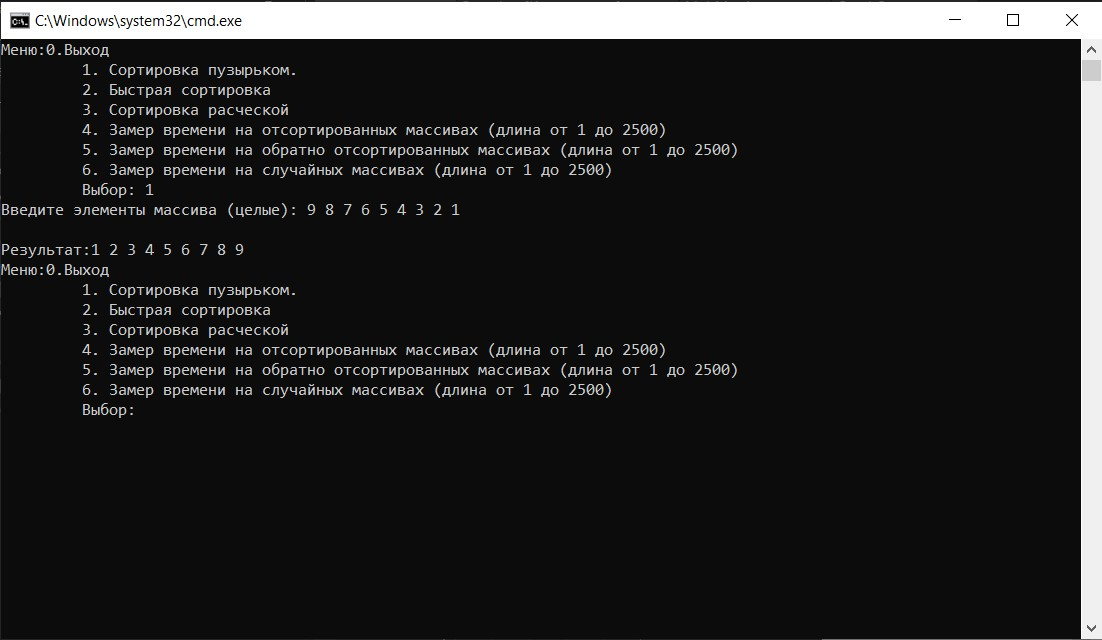
\includegraphics[width=1\linewidth]{inc/img/demob}
	\caption{Демонстрация работы реализации алгоритма сортировки пузырьком}
	\label{fig:demob}
\end{figure}

\begin{figure}[H]
	\centering
	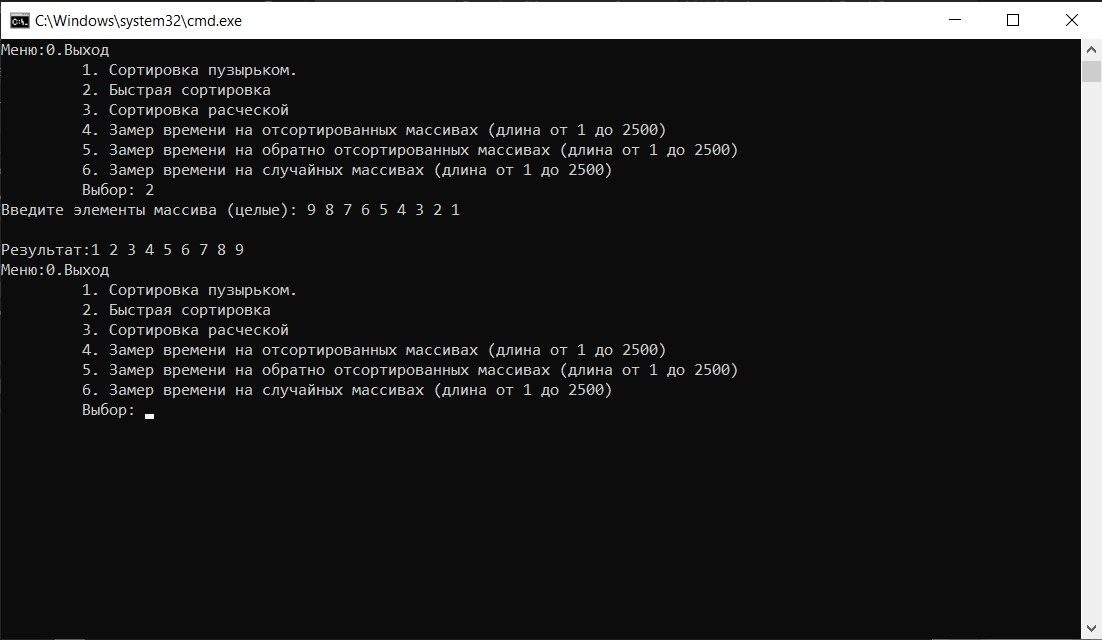
\includegraphics[width=1\linewidth]{inc/img/demoq}
	\caption{Демонстрация работы реализации алгоритма быстрой сортировки}
	\label{fig:demoq}
\end{figure}


\begin{figure}[H]
	\centering
	\includegraphics[width=1\linewidth]{"inc/img/Снимок экрана 2022-10-08 005524"}
	\caption{Демонстрация работы реализации алгоритма сортировки расческой}
	\label{fig:--2022-10-08-005524}
\end{figure}


\section{Время выполнения реализаций алгоритмов}

Время выполнения реализаций алгоритмов было замерено при помощи функции clock() \cite{cpplangtime}. Данная функция всегда возвращает значения времени, а именно сумму системного и пользовательского процессорного времени текущего процесса, значения типа float --- время в тиках.

Замеры времени для каждой длины массива проводились 100 раз. В качестве результата взято среднее время работы алгоритма на данной длине массива.

Результаты замеров приведены в таблицах \ref{tbl:best}, \ref{tbl:wor} и \ref{tbl:random} (время в тиках).
На рисунках \ref{fig:str}, \ref{fig:rev} и \ref{fig:rand}, приведены графики зависимостей времени работы алгоритмов сортировки от размеров массивов на отсортированных, обратно отсортированных и случайных данных.


\captionsetup{justification=raggedright, singlelinecheck=false}

\begin{table}[h]
	\begin{center}
		\caption{Время выполнения реализаций алгоритмов сортировки на отсортированных данных (время в тиках)}
		\label{tbl:best}
		\begin{tabular}{|c|c|c|c|}
			\hline
			 Размер & BubbleSort &  QuickSort &  CombSort \\
			\hline
			1&	0,01&	0&	0 \\
			\hline
			5&	0&	0&	0 \\
			\hline
			10&	0&	0&	0\\
			\hline
			50&	0,01&	0&	0\\
			\hline
			100&	0,04&	0,02&	0,01\\
			\hline
			500	&0,86&	0,61&	0,07\\
			\hline
			1000&	3,43&	2,41&	0,15\\
			\hline
			2000&	13,74&	9,57&	0,35\\
			\hline
			2500&	21,5&	14,93&	0,46\\
			\hline
		\end{tabular}
	\end{center}
	
\end{table}


\captionsetup{justification=centering, singlelinecheck=false}

\begin{figure}[H]
	\centering
	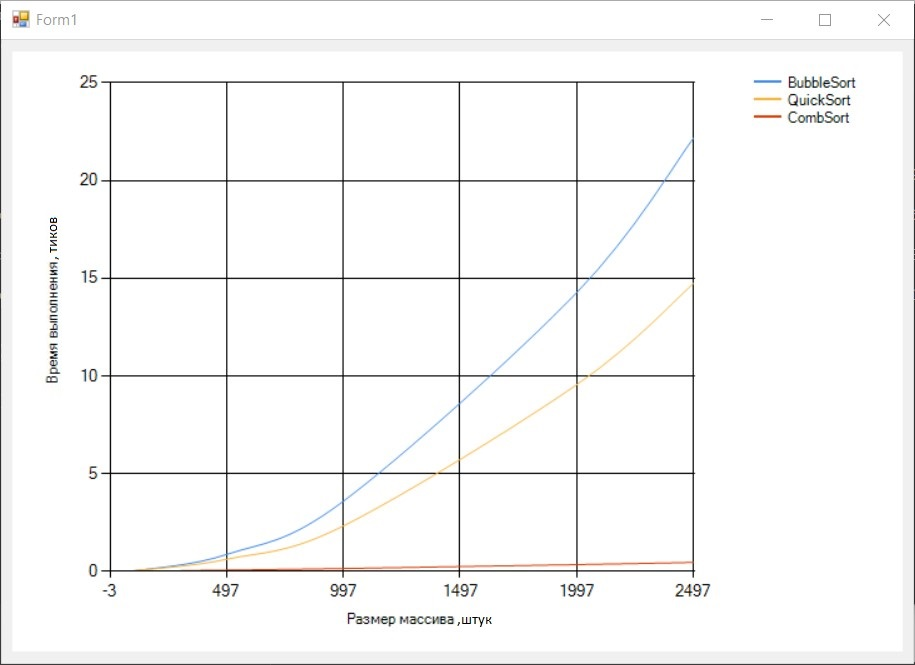
\includegraphics[width=0.7\linewidth]{inc/img/str}
	\caption{Зависимость времени сортировки отсортированного массива от размера массива (время в тиках)}
	\label{fig:str}
\end{figure}

\clearpage

\captionsetup{justification=raggedright, singlelinecheck=false}

\begin{table}[h]
	\begin{center}
		\caption{Время выполнения реализаций алгоритмов сортировки на обратно	отсортированных данных (время в тиках)}
		\label{tbl:wor}
		\begin{tabular}{|c|c|c|c|}
			\hline
			Размер & BubbleSort &  QuickSort &  CombSort \\
			\hline
			1&	0&	0&	0\\
			\hline
			5&	0&	0&	0\\
			\hline
			10&	0&	0&	0\\
			\hline
			50&	0,01&	0,01&	0\\
			\hline
			100&	0,04&	0,03&	0,01\\
			\hline
			500&	0,86&	0,61&	0,07\\
			\hline
			1000&	3,44&	2,4&	0,15\\
			\hline
			2000&	13,77&	9,52&	0,35\\
			\hline
			2500&	21,52&	14,86&	0,45\\
			\hline
		\end{tabular}
	\end{center}
	
\end{table}

\captionsetup{justification=centering, singlelinecheck=false}

\begin{figure}[H]
	\centering
	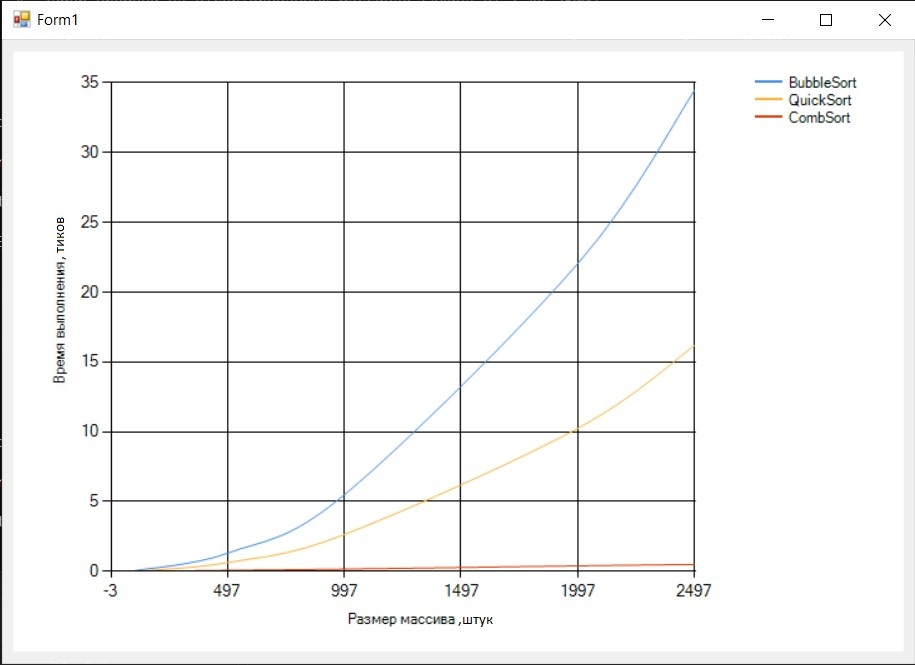
\includegraphics[width=0.7\linewidth]{inc/img/rev}
	\caption{Зависимость времени сортировки обратно отсортированного массива от размера массива (время в тиках)}
	\label{fig:rev}
\end{figure}

\clearpage

\captionsetup{justification=raggedright, singlelinecheck=false}

\begin{table}[h]
	\begin{center}
		\caption{Время выполнения реализаций алгоритмов сортировки на случайных данных (время в тиках)}
		\label{tbl:random}
		\begin{tabular}{|c|c|c|c|}
			\hline
			Размер & BubbleSort &  QuickSort &  CombSort \\
			\hline
			1&	0&	0,01&	0\\
			\hline
			5&	0,01&	0&	0\\
			\hline
			10&	0&	0&	0\\
			\hline
			50&	0,01&	0,01&	0\\
			\hline
			100&	0,05&	0,01&	0,02\\
			\hline
			500&	1,25&	0,06&	0,09\\
			\hline
			1000&	5,13&	0,14&	0,21\\
			\hline
			2000&	20,99&	0,33&	0,47\\
			\hline
			2500&	33,01&	0,4&	0,65\\
			\hline
		\end{tabular}
	\end{center}
	
\end{table}

\captionsetup{justification=centering, singlelinecheck=false}

\begin{figure}[H]
	\centering
	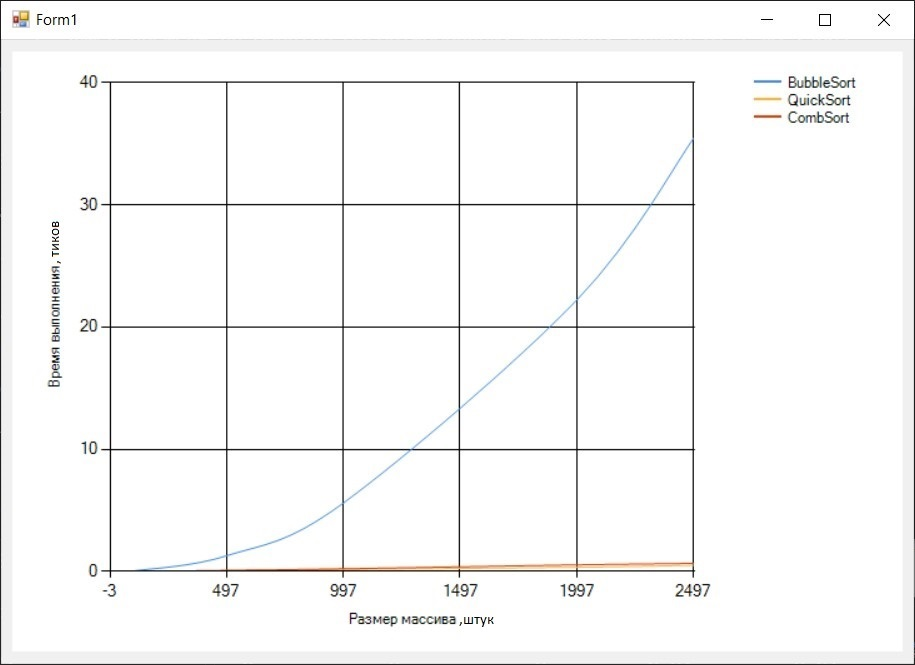
\includegraphics[width=0.7\linewidth]{inc/img/rand}
	\caption{Зависимость времени сортировки случайного массива от размера массива (время в тиках)}
	\label{fig:rand}
\end{figure}

\clearpage

\section*{Вывод}

%Алгоритм сортировки расческой работает быстрее остальных
%fixed
Реализация алгоритма сортировки расческой работает быстрее реализаций остальных алгоритмов при прямо и обратно отсортированных массивах.
Реализация алгоритма быстрой сортировки эффективнее по времени чем реализации двух других алгоритмов на массивах заполненных случайными числами.
Также реализация алгоритма быстрой сортировки работает значительно дольше, если массив отсортирован по убыванию или возрастанию.
%Реализация алгоритма сортировки расческой работает быстрее реализаций остальных алгоритмов в при отсортированных массивах, быстрой сортировки --- быстрее на случайных массивах.
%TODO: быстрая быстрее по отношении к чему? К себе на других данных или к другим реализациям всегда/в том же случае?

